% Supplementary report: OrchScope's orchestration engine on CAIDA's 2011 sipscan trace.
% Numbers, tables and figures are generated by code/sipscan_doc.py from results/ (none is typed
% by hand). Build: python code/sipscan_doc.py; cd docs; latexmk -pdf sipscan.tex
\documentclass[11pt]{article}
\usepackage[T1]{fontenc}
\usepackage{mathptmx}
\usepackage[margin=1in]{geometry}
\usepackage{graphicx,booktabs,amsmath}
\usepackage[font=small,labelfont=bf]{caption}
\usepackage{microtype}
\usepackage[hidelinks]{hyperref}
\usepackage{url}
\hypersetup{pdftitle={OrchScope on the 2011 Sipscan: Testing the Orchestration Engine on a
Documented Botnet Campaign}, pdfauthor={Elias Bou-Harb}}
% generated by code/sipscan_doc.py -- do not edit
\newcommand{\NoresAdd}{22}
\newcommand{\NoresBoth}{864}
\newcommand{\NoresDrop}{20}
\newcommand{\NoresGain}{42}
\newcommand{\NoresNegFlag}{0}
\newcommand{\NoresNegN}{8{,}000}
\newcommand{\NoresOrch}{906}
\newcommand{\NoresTestable}{8{,}363}
\newcommand{\NoresTzFlag}{0}
\newcommand{\NoresTzN}{7{,}443}
\newcommand{\OrionAllCountries}{19}
\newcommand{\OrionFive}{21{,}067}
\newcommand{\OrionOneHour}{18{,}845}
\newcommand{\OrionResidue}{18{,}793}
\newcommand{\OrionResiduePct}{89}
\newcommand{\OrionScanCountries}{6}
\newcommand{\OrionScanCountryList}{CN, DE, JP, MY, SG, US}
\newcommand{\OrionScanners}{2{,}274}
\newcommand{\OrionTopDest}{18{,}893}
\newcommand{\PaperNegN}{8{,}059}
\newcommand{\PaperTzN}{7{,}538}
\newcommand{\SipBots}{2{,}954{,}108}
\newcommand{\SipCheckBots}{3{,}000}
\newcommand{\SipCheckDmode}{2{,}999}
\newcommand{\SipCountries}{208}
\newcommand{\SipCountryCovPct}{3.8}
\newcommand{\SipCtlFlag}{5}
\newcommand{\SipCtlFlagDep}{18}
\newcommand{\SipCtlFlagDepPct}{1.1}
\newcommand{\SipCtlFlagPct}{0.3}
\newcommand{\SipCtlNactMed}{168}
\newcommand{\SipCtlOwnBH}{0}
\newcommand{\SipCtlOwnBHDep}{0}
\newcommand{\SipCtlOwnBHRot}{212}
\newcommand{\SipCtlOwnBHText}{none is flagged with either peer set}
\newcommand{\SipCtlPerSize}{320}
\newcommand{\SipCtlRotMax}{35}
\newcommand{\SipCtlTotal}{1{,}600}
\newcommand{\SipDeclineTime}{13:00 on Feb 6}
\newcommand{\SipDepBurst}{11:00 on Feb 12}
\newcommand{\SipDepOnsetAt}{00:00 on Feb 1}
\newcommand{\SipDepOnsetMax}{18}
\newcommand{\SipDepRestartAfter}{0}
\newcommand{\SipDepRestartAfterText}{never after it}
\newcommand{\SipDepRestartBefore}{97}
\newcommand{\SipDeployedMax}{0}
\newcommand{\SipDraws}{5}
\newcommand{\SipEarlyMax}{0}
\newcommand{\SipFallbackPct}{96}
\newcommand{\SipFallbackPctDep}{68}
\newcommand{\SipFullPopFirst}{0}
\newcommand{\SipFullPopLast}{53}
\newcommand{\SipFullRotFirst}{9}
\newcommand{\SipFullRotFrom}{Feb 4}
\newcommand{\SipFullRotLast}{100}
\newcommand{\SipFullTestable}{0}
\newcommand{\SipIdleDays}{5.0}
\newcommand{\SipIdleHi}{238}
\newcommand{\SipIdleLo}{65}
\newcommand{\SipNactMed}{2}
\newcommand{\SipOnsetAll}{23:00 on Jan 31}
\newcommand{\SipOnsetCamps}{14}
\newcommand{\SipOnsetFirstUpdate}{22:00 on Jan 31}
\newcommand{\SipOnsetFlag}{14}
\newcommand{\SipOnsetLastTestable}{14:00 on Feb 1}
\newcommand{\SipOnsetSubPct}{91}
\newcommand{\SipOnsetTime}{21:07 on Jan 31}
\newcommand{\SipPackets}{20{,}255{,}721}
\newcommand{\SipPeakSlice}{8{,}051}
\newcommand{\SipPerCell}{160}
\newcommand{\SipPerSize}{1{,}280}
\newcommand{\SipProfMax}{71{,}379}
\newcommand{\SipProfMin}{23{,}692}
\newcommand{\SipReplayUpdates}{293}
\newcommand{\SipRestartDelay}{10}
\newcommand{\SipRestartFirst}{32}
\newcommand{\SipRestartFirstUpdate}{00:00 on Feb 12}
\newcommand{\SipRestartFullTestable}{0}
\newcommand{\SipRestartHours}{25}
\newcommand{\SipRestartSlices}{32}
\newcommand{\SipRestartTime}{14:00 on Feb 11}
\newcommand{\SipRotEarlyMin}{13}
\newcommand{\SipSevenHundred}{98}
\newcommand{\SipSevenThirty}{82}
\newcommand{\SipSevenThousand}{100}
\newcommand{\SipSixThirty}{26}
\newcommand{\SipSixThousand}{70}
\newcommand{\SipSliceWindows}{256}
\newcommand{\SipSlices}{32}
\newcommand{\SipSteadyDays}{5.7}
\newcommand{\SipSteadyFlagged}{1}
\newcommand{\SipSteadyRotMax}{81}
\newcommand{\SipSteadySliceUpdates}{3{,}872}
\newcommand{\SipSteadyUpdates}{121}
\newcommand{\SipStopTime}{15:00 on Feb 12}
\newcommand{\SipTau}{0.0043}
\newcommand{\SipTauRot}{0.0257}
\newcommand{\SipWindows}{8}
\newcommand{\WeekOrch}{884}
\newcommand{\WeekTestable}{8{,}781}
\newcommand{\WeekTested}{10{,}398}

\newcommand{\sysname}{OrchScope}
\renewcommand{\floatpagefraction}{0.8}

\title{\sysname{} on the 2011 Sipscan:\\Testing the Orchestration Engine on a Documented Botnet
Campaign}
\author{Elias Bou-Harb\\[2pt]
\normalsize Division of Computer Science and Engineering, Louisiana State University,
Baton Rouge, LA, USA\\
\normalsize \texttt{ebouharb@lsu.edu}}
\date{\normalsize Supplementary report to \emph{``OrchScope: A Calibrated, Near-Real-Time System to
Infer Orchestrated Scanning Campaigns at a Network Telescope''} (submitted to IEEE ICC 2027).\\
October 2026}

\begin{document}
\maketitle

\begin{abstract}
\sysname's orchestration engine decides whether a campaign of co-tooled scanners is
orchestrated, that is, more synchronized than independent operation explains. The paper
validates it on simulated campaigns and on random groups of real sources; neither is a real
orchestrated campaign. This report tests it on one: the sipscan, a scan of the entire IPv4 space
for SIP servers that the Sality botnet ran under central command in February 2011, as captured by
the UCSD Network Telescope and released by CAIDA. We replay the scan through ORION-sized views of
that telescope, with the paper's test and decision threshold and with peers borrowed from ORION's
port-5060 sources. With the port's scanners as peers, the engine flags the botnet within an hour
of its onset and flags its restart at the first decision its weekly window allows, but not the
\SipSteadyDays-day steady phase in between, whose timing matches independent scanning. Random
groups of ORION's scanners are flagged \SipCtlFlag{} times in \SipCtlTotal. The replay also
exposes a limitation: as deployed, the population null also draws peers from residue sources, and
on ORION's port 5060, where \OrionResiduePct\% of the sources form one residue event, it can flag
nothing. Excluding residue sources from the peer pools changes the paper's week from \WeekOrch{}
to \NoresOrch{} orchestrated campaigns, and both of its negative controls still flag none.
\end{abstract}

\section{Introduction}

\sysname~\cite{orchscope} infers scanning campaigns at the Merit ORION network
telescope~\cite{ismail2025merit} and decides, for each campaign, whether its sources are
orchestrated: whether they act together more tightly than independent operation explains. Its
orchestration engine (Section~III-C of the paper) compares a campaign's mean pairwise
co-activity with two nulls and declares the campaign orchestrated only if both reject. The paper
evaluates the engine on synthetic campaigns injected into real background traffic, where the
schedule of every bot is known, and on random groups of real sources, which should not be
flagged. Both are needed, but neither is a real orchestrated campaign observed in the wild.

This report supplies one. In February 2011, the Sality botnet scanned the entire IPv4 address
space for SIP servers (UDP port 5060) under the control of its command-and-control (C\&C)
infrastructure. The scan, known as the sipscan, reached the UCSD Network Telescope from about
three million bots; Dainotti et al.\ analyze it in
detail~\cite{dainotti2012imc,dainotti2015ton}, and CAIDA releases every sipscan probe that reached
the telescope~\cite{caida_sipscan}. We replay this campaign through \sysname's orchestration engine
at ORION's scale and ask four questions:
\begin{enumerate}
\item Does the engine flag a real, centrally commanded campaign, and in which of its phases?
\item How soon does it flag it when run hour by hour, as deployed?
\item How often, under the same settings, does it flag random groups of real scanners on the
same port?
\item What does the replay reveal about the engine itself?
\end{enumerate}
Section~\ref{sec:data} describes the data, Section~\ref{sec:method} the method,
Section~\ref{sec:results} the results and Section~\ref{sec:meaning} what they show;
Section~\ref{sec:threats} discusses threats to validity and Section~\ref{sec:repro} reproduction
and data use.

\section{The Sipscan Data}
\label{sec:data}

CAIDA's Sipscan Dataset~\cite{caida_sipscan} holds one row per sipscan probe that reached the
UCSD Network Telescope, a /8 darknet: \SipPackets{} UDP packets to port 5060 from \SipBots{}
sources in \SipCountries{} countries, between January 31 and February 14, 2011. Each row gives
the arrival time, the source's country, coordinates and autonomous system, an anonymized source
identifier (one to one with the source address), the destination address with its first octet
replaced, and the source port. There are no other header fields, and the dataset holds no traffic
other than the sipscan's: every source in it is a sipscan bot.

Figure~\ref{fig:timeline} (top) shows the campaign as an ORION-sized telescope sees it: the
distinct bots per hour within one /13 of the /8 (Section~\ref{sec:views}), averaged over the 32
such slices. The bots started within minutes at \SipOnsetTime{} (all times UTC) and scanned for
\SipSteadyDays{} days with a daily rhythm. From \SipDeclineTime{} their number fell within a day
to a trickle of \SipIdleLo--\SipIdleHi{} bots per hour per slice. At \SipRestartTime, \SipIdleDays{}
days after the decline began, the botnet restarted at full strength, peaking at \SipPeakSlice{}
bots per hour per slice, and it stopped abruptly at \SipStopTime, \SipRestartHours{} hours later.
The
near-simultaneous start, restart and stop of a whole botnet are the kind of command that a test of
synchrony should see; the steady phase in between is the hard case.

\begin{figure}[t]
\centering
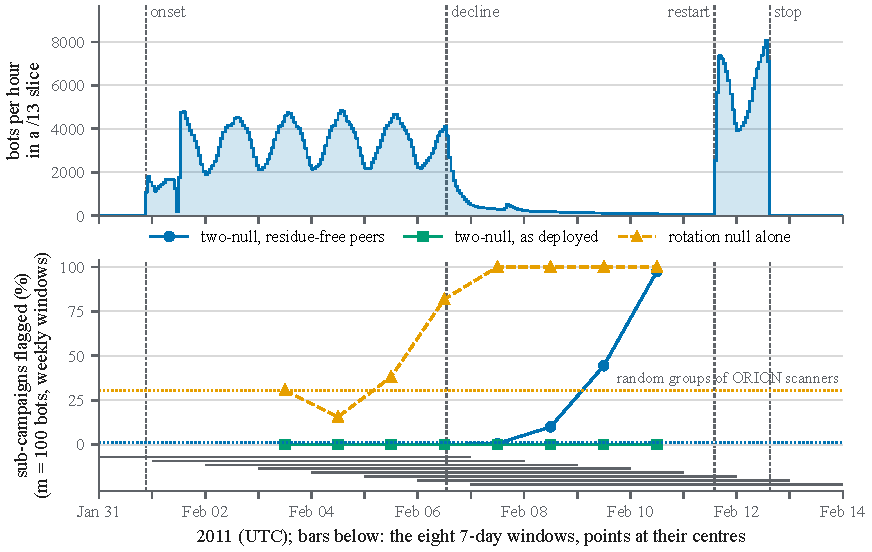
\includegraphics[width=\linewidth]{sipscan_timeline.pdf}
\caption{Top: the sipscan as an ORION-sized telescope sees it, as distinct bots per hour in a /13
of the UCSD /8 (mean of the 32 slices); dashed lines mark the onset, the decline, the restart and
the stop. Bottom: share of 100-bot sub-campaigns flagged in each 7-day window (bars below the
axis; points at their centres) by the two-null test with residue-free peers, by the two-null test
with all port-5060 peers as deployed, and by the rotation null alone. Dotted lines: random groups
of ORION's scanners, two-null test with residue-free peers and rotation null alone.}
\label{fig:timeline}
\end{figure}

\section{Method}
\label{sec:method}

\subsection{Scope}
Without header fields there is no tool fingerprint, so \sysname's inference engine, which blocks
sources by port and fingerprint before clustering them, cannot be evaluated here. We test the
orchestration engine alone, on groups whose membership is known: every source of the dataset
belongs to the sipscan.

\subsection{ORION-sized views}
\label{sec:views}
ORION monitors a /13, about half a million addresses. A /8 holds 32 /13s, so we split the
telescope into 32 slices by the first five bits of the destination's second octet, which the
dataset keeps intact; each slice is an ORION-sized view of the same campaign. Within a slice, a
bot is profiled once it has sent two packets there: \sysname{} profiles sources with at least two
distinct destinations or two packet samples, and a source with two packets has one or the other.
For each profiled bot we build the fields that the orchestration engine reads: its hourly
activity bitmap over the test window, its number of active hours, its country, and its modal
destination, which the residue rule uses. To check this shortcut, we rebuilt \SipCheckBots{} bots
of one slice and window through the production path: ORION-format flow records, one per bot, hour
and port, each with up to three packet samples carrying the real destination and source port, fed
to the production reducer and profiler. Active hours, countries and ports agreed for all
\SipCheckBots{} bots, and the modal destination for \SipCheckDmode.

\subsection{The test, as in the paper}
Every group is tested as in the paper. The statistic is the mean Jaccard co-activity of the
members' hourly bitmaps over at most 600 sampled member pairs. The rotation null shifts each
member's bitmap circularly by an independent whole number of days~\cite{lancaster2018surrogate};
the population null replaces each member with a random non-member of the same port and country
(of the port alone if the country has fewer than 40) in the same power-of-two bin of active
hours. Each null yields an exact Monte Carlo $p$-value from 200 surrogates, refined with 1,000
fresh surrogates if $p\le0.1$ and with $10^4$ if $p\le0.01$; the two-null $p$-value is the larger
of the two, an intersection--union test~\cite{berger1982iut}. A group whose port has fewer
non-members than members is not tested, and its orchestration is undetermined. Weekly windows
span 168 hours.

\subsection{Peers borrowed from ORION}
\label{sec:peers}
The population null needs the campaign's port peers, and the dataset has none. We borrow them
from the paper's ORION week (September 24--30, 2026): the \OrionFive{} sources whose primary port
is 5060. One event dominates that population: \OrionResidue{} of its sources (\OrionResiduePct\%)
belong to groups that \sysname{} sets aside as residue, \OrionTopDest{} share one modal dark
destination, and \OrionOneHour{} were active in the same single hour. \sysname{} never tests
residue groups, but as deployed it still draws peers from their sources. We therefore run every
experiment with two peer sets: all \OrionFive{} sources, as deployed (\emph{Dep.}), and the
\OrionScanners{} sources outside residue groups (\emph{residue-free}, RF). Only
\OrionScanCountries{} countries (\OrionScanCountryList) have 40 or more residue-free sources on the
port, and they hold \SipCountryCovPct\% of the sipscan's bots, so for \SipFallbackPct\% of the
bots the population null draws peers from the whole port. Both datasets keep UTC timestamps, so
hours of the day align; in the hourly replay (Section~\ref{sec:replay}), days of the week align
too.

\subsection{Decision threshold}
A group is flagged if Benjamini--Hochberg (BH) at $q=0.05$~\cite{benjamini1995fdr} would flag it
when its $p$-value joins the \WeekTested{} $p$-values that the paper's week tested, that is, if
$p\le\SipTau$. For the rotation null alone, joining the week's rotation $p$-values, the threshold
is $p\le\SipTauRot$. Each group thus faces the decision of a deployment in which the sipscan
appears among ORION's real campaigns.

\subsection{Experiment 1: weekly windows}
We use \SipWindows{} weekly windows of 168 hours, starting at 00:00 on each day from January 31
to February 7, in all \SipSlices{} slices. A slice holds \SipProfMin{} to \SipProfMax{} profiled bots per window
(medians across slices). At that size the sipscan outnumbers its peers in every slice and window,
so \sysname{} would report it as undetermined; we test it whole with that rule waived, and we test
sub-campaigns of $m=10$, 30, 100, 300 and 1,000 bots drawn at random within a slice and window,
\SipDraws{} per size, slice and window (\SipPerSize{} per size). For scale, the median
orchestrated campaign in the paper's week has 30 sources.

\subsection{Experiment 2: negative controls}
Random groups of ORION's residue-free port-5060 sources, \SipCtlPerSize{} per size and
\SipCtlTotal{} in all, go through the same test, peers and threshold. (Random groups of residue sources are
themselves residue, which \sysname{} never tests.) We also apply BH to the controls' own
$p$-values, as the paper's negative control does.

\subsection{Experiment 3: hourly replay}
\label{sec:replay}
As deployed, \sysname{} updates its campaigns after every hourly batch over a weekly landmark
window; the test sees the most recent whole days ending at the current hour, and decisions start
once two whole days exist. ORION's week starts on a Thursday, and so do the three windows we
replay: from January 27, whose fifth day holds the onset; from February 3, which holds steady
scanning and the decline; and from February 10, whose second and third days hold the restart and
the stop. At each hourly update from the end of day two to the end of day seven (121 updates per
window), the campaign of a slice is every bot profiled in that slice so far; it needs ten members
and is testable while its port has at least as many peers as it has members. We also test a
random 30-bot sub-campaign of it. The peers are the ORION sources active by the same hour of
ORION's week, with their bitmaps cut to the same trailing days.

\subsection{Experiment 4: residue-free peers on the paper's week}
To measure what excluding residue sources from the peer pools would change in the paper, we
re-test the week's \WeekTested{} campaigns with residue-free pools, on the pipeline's own
per-campaign surrogate seeds, and re-run both negative controls of the paper (same port; same
port and country).

\section{Results}
\label{sec:results}

\subsection{Weekly windows}
Table~\ref{tab:windows} and Fig.~\ref{fig:timeline} (bottom) give the flagged share per window.
With all port-5060 sources as peers, as deployed, no sipscan sub-campaign is flagged in any window
or at any size (\SipDeployedMax\%): against peers this synchronized, the population null cannot
reject. With residue-free peers, the two-null test flags the sipscan in the windows where its bots
switched on and off: \SipSevenThirty\% of 30-bot and \SipSevenHundred\% of 100-bot sub-campaigns
in the window from February 7, which holds the restart and the stop but no steady scanning, and
\SipSixThirty--\SipSixThousand\% in the window from February 6. In the four windows that the
steady phase dominates, from January 31 to February 3, it flags none (\SipEarlyMax\%). A weekly
window also dilutes the onset, which the window from January 31 holds together with
\SipSteadyDays{} days of steady scanning; the hourly replay isolates it (Section~\ref{sec:res:replay}).
The rotation null alone flags \SipRotEarlyMin--100\% of the sipscan's sub-campaigns, depending on
the window.

\begin{table}[t]
\centering
\caption{Sipscan sub-campaigns flagged per 7-day window, in percent of \SipPerCell{} per cell: the
two-null test with residue-free peers (RF) and with all port-5060 peers as deployed (Dep.), and
the rotation null alone (Rot.). ``Holds'': phases of the scan inside the window.}
\label{tab:windows}
\small
\setlength{\tabcolsep}{3.6pt}
% generated by code/sipscan_doc.py -- do not edit
\begin{tabular}{@{}llrrrrrrrrr@{}}
\toprule
 & & \multicolumn{3}{c}{$m=30$} & \multicolumn{3}{c}{$m=100$} & \multicolumn{3}{c}{$m=1{,}000$} \\
\cmidrule(lr){3-5}\cmidrule(lr){6-8}\cmidrule(l){9-11}
Window from & Holds & RF & Dep. & Rot. & RF & Dep. & Rot. & RF & Dep. & Rot. \\
\midrule
Jan 31 & onset, steady, decline & 0 & 0 & 19 & 0 & 0 & 31 & 0 & 0 & 22 \\
Feb 1 & steady, decline, idle & 0 & 0 & 13 & 0 & 0 & 16 & 0 & 0 & 17 \\
Feb 2 & steady, decline, idle & 0 & 0 & 28 & 0 & 0 & 38 & 0 & 0 & 46 \\
Feb 3 & steady, decline, idle & 0 & 0 & 74 & 0 & 0 & 82 & 0 & 0 & 89 \\
Feb 4 & steady, decline, idle & 0 & 0 & 93 & 1 & 0 & 100 & 1 & 0 & 99 \\
Feb 5 & steady, decline, idle, restart & 2 & 0 & 98 & 10 & 0 & 100 & 21 & 0 & 100 \\
Feb 6 & steady, decline, idle, restart, stop & 26 & 0 & 100 & 44 & 0 & 100 & 70 & 0 & 100 \\
Feb 7 & decline, idle, restart, stop & 82 & 0 & 100 & 98 & 0 & 100 & 100 & 0 & 100 \\
\bottomrule
\end{tabular}

\end{table}

Taken whole, the sipscan is undetermined in all \SipSliceWindows{} slice-windows
(\SipFullTestable{} testable), as it outnumbers the port's peers. With that rule waived, the
population null rejects in \SipFullPopFirst\% of the slices in the window from January 31 and in
\SipFullPopLast\% in the window from February 7; the rotation null alone rejects in
\SipFullRotFirst\% and \SipFullRotLast\%, and in every slice from the window of \SipFullRotFrom{}
on.

\subsection{Negative controls}
Table~\ref{tab:sizes} pools the windows by size. Random groups of ORION's port-5060 scanners are
flagged \SipCtlFlag{} times in \SipCtlTotal{} (\SipCtlFlagPct\%) with residue-free peers and
\SipCtlFlagDep{} times (\SipCtlFlagDepPct\%) as deployed. With BH applied to the controls alone, as
in the paper, \SipCtlOwnBHText. The rotation null alone flags up
to \SipCtlRotMax\% of them at the deployment threshold, and \SipCtlOwnBHRot{} of \SipCtlTotal{}
under their own BH: alone, it cannot tell the sipscan from the port's independent scanners. The
controls' members are mostly always-on scanners (median \SipCtlNactMed{} active hours of 168,
against \SipNactMed{} for the sipscan's bots), as is the port's residue-free population.

\begin{table}[t]
\centering
\caption{Flagged share in percent, over all eight windows, by group size: sipscan sub-campaigns
(``sipscan'') and random groups of ORION's residue-free port-5060 sources, under the same test, peers and
threshold (RF: residue-free peers; Dep.: all port-5060 peers, as deployed; Rot.: rotation null
alone).}
\label{tab:sizes}
\small
% generated by code/sipscan_doc.py -- do not edit
\begin{tabular}{@{}rrrrrrr@{}}
\toprule
 & \multicolumn{3}{c}{sipscan} & \multicolumn{3}{c}{random groups} \\
\cmidrule(lr){2-4}\cmidrule(l){5-7}
$m$ & RF & Dep. & Rot. & RF & Dep. & Rot. \\
\midrule
10 & 1.4 & 0.0 & 30.3 & 0.0 & 0.0 & 2.2 \\
30 & 13.7 & 0.0 & 65.6 & 0.3 & 0.9 & 18.8 \\
100 & 19.1 & 0.0 & 70.8 & 1.2 & 1.9 & 30.6 \\
300 & 22.3 & 0.0 & 70.3 & 0.0 & 1.2 & 31.6 \\
1{,}000 & 24.0 & 0.0 & 71.6 & 0.0 & 1.6 & 35.3 \\
\midrule
groups per row & \multicolumn{3}{c}{1{,}280} & \multicolumn{3}{c}{320} \\
\bottomrule
\end{tabular}

\end{table}

\subsection{Hourly replay}
\label{sec:res:replay}
Figure~\ref{fig:stream} shows the share of slices whose 30-bot sub-campaign is flagged at each
hourly update. With residue-free peers the onset is caught at once. At the first update after it,
at \SipOnsetFirstUpdate, \SipOnsetCamps{} slices already hold a campaign of ten or more bots and
\SipOnsetFlag{} of them are flagged; from \SipOnsetAll{} on, all 32 are. The whole campaign stays
testable until \SipOnsetLastTestable, when it outgrows its peers and becomes undetermined, while
its 30-bot sub-campaigns stay flagged in \SipOnsetSubPct\% of the slice-updates to the window's
end. In the window from February 3, \SipSteadyFlagged{} of \SipSteadySliceUpdates{} slice-updates
flags a sub-campaign, whereas the rotation null alone flags up to \SipSteadyRotMax\% of them once
the decline enters the window. The restart falls on day two of its window, so the first decision
comes at \SipRestartFirstUpdate, \SipRestartDelay{} hours after it; that decision flags the 30-bot
sub-campaigns in \SipRestartFirst{} of \SipRestartSlices{} slices, while the whole campaign is by
then undetermined.

As deployed, with all port-5060 peers, the onset is flagged in at most \SipDepOnsetMax{} of 32
slices (at \SipDepOnsetAt). The restart is flagged in \SipDepRestartBefore\% of slice-updates until
\SipDepBurst, the hour of ORION's week at which its residue event enters the peer pool, and
\SipDepRestartAfterText. That the restart's first decisions precede the event is a
coincidence of aligning 2011 with ORION's week.

\begin{figure}[t]
\centering
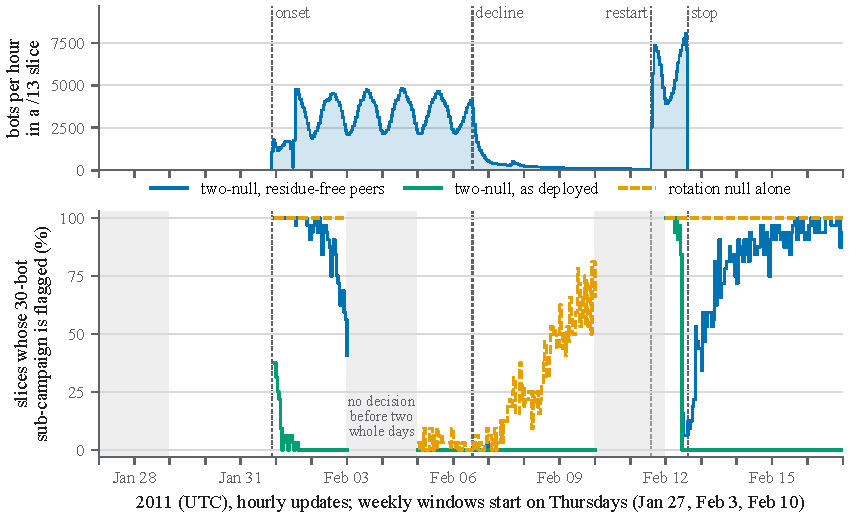
\includegraphics[width=\linewidth]{sipscan_stream.pdf}
\caption{Hourly replay in the deployment mode. Top: as in Fig.~\ref{fig:timeline}. Bottom: share of
the 32 slices whose 30-bot sub-campaign is flagged at each hourly update of the three Thursday
windows; shaded: the first two days of each window, when no decision is made.}
\label{fig:stream}
\end{figure}

\subsection{Residue-free peers on the paper's week}
Table~\ref{tab:nores} re-tests the paper's week with residue-free peer pools. Fewer campaigns are
testable (\NoresTestable{} instead of \WeekTestable), since some ports lose peers, and
\NoresOrch{} campaigns are orchestrated instead of \WeekOrch: \NoresBoth{} are flagged either way,
\NoresDrop{} only as deployed and \NoresGain{} only with residue-free peers. Both negative controls
still flag none, with practically unchanged uncorrected rejection rates.

\begin{table}[t]
\centering
\caption{The paper's week re-tested with residue-free peer pools, on the pipeline's own surrogate
draws, and the paper's two negative controls re-run with those pools.}
\label{tab:nores}
\small
% generated by code/sipscan_doc.py -- do not edit
\begin{tabular}{@{}lrr@{}}
\toprule
 & Paper (as deployed) & Residue-free peers \\
\midrule
Testable campaigns & 8{,}781 & 8{,}363 \\
Orchestrated (BH, $q=0.05$) & 884 & 906 \\
\quad flagged by both & 864 & 864 \\
\quad TCP / UDP & 465 / 330 & 477 / 341 \\
Same-port control: flagged / groups & 0 / 8{,}059 & 0 / 8{,}000 \\
\quad uncorrected $p<0.05$ / $p<0.01$ & 2.8\% / 0.5\% & 2.7\% / 0.5\% \\
Same-country control: flagged / groups & 0 / 7{,}538 & 0 / 7{,}443 \\
\quad uncorrected $p<0.05$ / $p<0.01$ & 3.1\% / 0.7\% & 2.8\% / 0.6\% \\
\bottomrule
\end{tabular}

\end{table}

\section{What the Sipscan Shows}
\label{sec:meaning}

\paragraph{The engine detects commanded synchrony.} The two-null test flags a real
C\&C-orchestrated campaign where the C\&C switched its bots on or off together: within an hour of
the sipscan's onset at ORION's scale, and at the first decision after its restart. This is the
synchrony the test is built to find, and the replay shows it on a real botnet rather than a
simulated one.

\paragraph{A steady phase is invisible to a timing test.} During its \SipSteadyDays{} days of
steady scanning, each bot appears in an ORION-sized view for about two hours, and the botnet's
volume follows the same daily rhythm every day. Its timing then matches that of independent
scanners, and no test of synchrony can separate the two; whatever coordinated the bots in this
phase did not show in when they ran. For such campaigns \sysname{} reports the campaign without
the orchestration flag, so ``not orchestrated'' means ``no evidence of synchrony'', not
``independent''.

\paragraph{The rotation null alone is not enough.} It flags much of the sipscan, but also up to
\SipCtlRotMax\% of random groups of the port's scanners, as the paper's negative controls found
across all ports.

\paragraph{Peer pools should exclude residue sources.} As deployed, the population null includes
them. On a port that one residue event dominates, it then compares every campaign with peers more
synchronized than any scanner, and here it hid every sipscan sub-campaign. Excluding residue
sources keeps both of the paper's negative controls clean and changes its week by \NoresAdd{}
orchestrated campaigns (Table~\ref{tab:nores}).

\section{Threats to Validity}
\label{sec:threats}

\paragraph{Transplanted peers.} The peers come from ORION in 2026 and the sipscan from UCSD in
2011; their port-5060 populations differ, and the residue event of ORION's week is specific to
that week. Other peer populations could change the results.

\paragraph{Sub-campaigns.} The tested groups are random subsets of one botnet, not groups formed by
\sysname's blocking and clustering, which the dataset cannot exercise; taken whole, the campaign is
untestable at ORION's scale.

\paragraph{Dependence between slices.} The 32 slices are views of the same bots, not independent
replicates; the flagged shares describe the spread across views, not independent trials.

\paragraph{One campaign, one scale.} All results hold for one campaign and one telescope size
(/13). Weekly windows align hours of the day between 2011 and 2026, and the replay also aligns
days of the week; the as-deployed restart result depends on that alignment.

\section{Reproduction and Data Use}
\label{sec:repro}

All code and aggregate results are in the OrchScope repository,
\url{https://github.com/ebh2024ebh/orchscope}:
\begin{itemize}
\item \path{code/sipscan_eval.py}: the analysis, with subcommands \texttt{prep}, \texttt{check},
\texttt{week} and \texttt{stream}, run next to the paper's week profiles (Experiments 1--3);
\item \texttt{code/revision\_checks.py nores}: Experiment~4;
\item \path{code/sipscan_timeline.py}: the hourly counts of Fig.~\ref{fig:timeline};
\item \path{code/sipscan_doc.py}: this report's figures, tables and numbers, from the aggregate
results in \path{results/}; no number is typed by hand.
\end{itemize}
All random draws use fixed seeds, so reruns reproduce every number.

The sipscan data are used under CAIDA's Acceptable Use Agreement for publicly accessible datasets
and are not redistributed; the released files hold aggregates only. ORION traffic was analyzed
passively under a data-use agreement with Merit Network and is not redistributed either.

\bibliographystyle{IEEEtran}
\bibliography{sipscan}

\end{document}
